% 16:9 Beamer
\documentclass[10pt, aspectratio=169]{beamer}

% Packages
\usepackage[greek,english]{babel}
\usepackage{amsmath, amssymb, graphicx}
\usepackage{alphabeta, booktabs, subcaption, array}

% Aesthetics
\usetheme{metropolis}
\metroset{block=fill}   % block background

% Color Palette
\definecolor{ntuablue}{RGB}{0, 51, 102}
\definecolor{medicalblue}{RGB}{30, 113, 190}
\definecolor{accentorange}{RGB}{230, 126, 34}
\definecolor{lightgray}{RGB}{245, 245, 245}

% Beamer Elements Colors
\setbeamercolor{palette primary}{bg=ntuablue, fg=white}
\setbeamercolor{frametitle}{bg=ntuablue, fg=white}
\setbeamercolor{progress bar}{fg=accentorange, bg=lightgray}
\setbeamercolor{block title}{bg=medicalblue, fg=white}
\setbeamercolor{block body}{bg=lightgray, fg=black}
\setbeamercolor{alerted text}{fg=accentorange}

% Custom Title Page
\setbeamertemplate{title page}{\begin{minipage}[b][\paperheight]{\textwidth}\color{white}\vspace*{25pt}
{\footnotesize\insertinstitute}\par\vspace*{15pt}
{\Large\bfseries\inserttitle}\par\vspace*{10pt}
{\small\insertsubtitle}\par\vspace*{15pt}
{\color{accentorange}\rule{\textwidth}{1pt}}\par\vspace*{15pt}
{\small\insertauthor}\par\vspace*{12pt}
{\footnotesize \insertdate}\par\vspace*{25pt}
\end{minipage}}

% Presentation Metadata
\title{Physically Interpretable World Models\vspace{-0.125cm}}
\subtitle{Four Principles for Physically Interpretable World Models\\ {\scriptsizeΑναπαραγωγή, Αξιολόγηση \& Επεκτάσεις}\\[0.375cm] \largeΤελική Παρουσίαση\vspace{-0.375cm}}
\author{\vspace{-0.25cm}Ακαδημαϊκό έτος 2025-2026\vspace{-0.25cm}}
\institute{Εθνικό Μετσόβιο Πολυτεχνείο\\ Σχολή Ηλεκτρολόγων Μηχανικών \& Μηχανικών Υπολογιστών\\ Συστήματα Λήψης και Απόφασης\\ Εξαμηνιαία Εργασία\vspace{-0.125cm}}
\date{Ιούνιος 2026}

\begin{document}

% Slide 0 : Title Page
{\setbeamercolor{background canvas}{bg=ntuablue}
\setbeamercolor{normal text}{fg=white}
\maketitle}

% ==========================================
% SECTION 1: ΣΥΝΟΨΗ ΤΟΥ PAPER (1-2 διαφάνειες)
% ==========================================

% Slide 1 : Paper Summary 1 - Introduction & Interpretable World Models
\begin{frame}{Σύνοψη Paper: Φυσική Ερμηνευσιμότητα στα \textlatin{World Models}}
    \footnotesize Τα \textlatin{World Models} μαθαίνουν τη δυναμική του περιβάλλοντος από \textlatin{pixels}, αλλά ο λανθάνων χώρος τους είναι συνήθως «μαύρο κουτί».
    \par\vspace{0.15cm}
    \begin{columns}[onlytextwidth, T]
        \begin{column}{0.48\textwidth}
            \begin{block}{Το Πρόβλημα}
                \begin{itemize}
                    \item \scriptsize \textbf{Physically Informed:} Η φυσική γνώση εισάγεται ως \textlatin{loss regularizer}, αλλά ο λανθάνων χώρος παραμένει αδιαφανής.
                    \item \scriptsize Δεν υπάρχουν φυσικές εγγυήσεις, ούτε δυνατότητα άμεσης σύνδεσης με κλασικό έλεγχο (\textlatin{PID}, \textlatin{MPC}) ή τυπική επαλήθευση.
                \end{itemize}
            \end{block}
        \end{column}
        \begin{column}{0.48\textwidth}
            \begin{block}{Η Προτεινόμενη Λύση (PIWM)}
                \begin{itemize}
                    \item \scriptsize Ο λανθάνων χώρος αποκτά \textbf{ρητό φυσικό νόημα} (π.χ. συγκεκριμένες διαστάσεις αντιστοιχούν σε θέση, γωνία, ταχύτητα).
                    \item \scriptsize Επιτυγχάνεται αξιοπιστία, ευκολότερος εντοπισμός σφαλμάτων και άμεση διεπαφή με συστήματα ελέγχου.
                \end{itemize}
            \end{block}
        \end{column}
    \end{columns}
\end{frame}

% Slide 2 : Paper Summary 2 - The Four Principles
\begin{frame}{Σύνοψη Paper: Οι Τέσσερις Αρχές Σχεδιασμού}
    \footnotesize Οι συγγραφείς προτείνουν 4 θεμελιώδεις αρχές για την κατασκευή φυσικά ερμηνεύσιμων μοντέλων:\par\vspace{0.2cm}
    \begin{columns}[onlytextwidth, T]
        \begin{column}{0.48\textwidth}
            \begin{block}{Αρχή 1: Δομική Αποσύνδεση}
                \scriptsize \textbf{Ιδέα:} Διαχωρισμός του \textlatin{latent space} σε φυσική κατάσταση $z_{\text{\textlatin{phys}}}$ και οπτικό στυλ $z_{\text{\textlatin{img}}}$.
                \[ z = [E_{\text{phys}}(o), E_{\text{img}}(o)] \]
            \end{block}
            \begin{block}{Αρχή 2: Equivariance \& Invariance}
                \scriptsize \textbf{Ιδέα:} Οπτικές αλλαγές (π.χ. φωτισμός) δεν πρέπει να επηρεάζουν τη φυσική κατάσταση.
                \[ E(g \cdot o) \approx h \cdot E(o) \]
            \end{block}
        \end{column}
        \begin{column}{0.48\textwidth}
            \begin{block}{Αρχή 3: Πολυεπίπεδη Επίβλεψη}
                \scriptsize \textbf{Ιδέα:} Σύνδεση των διαστάσεων του $z_{\text{\textlatin{phys}}}$ με πραγματικά φυσικά μεγέθη μέσω πλήρους, ασθενούς ή αυτο-επίβλεψης.
            \end{block}
            \begin{block}{Αρχή 4: Διαμέριση Εξόδου}
                \scriptsize \textbf{Ιδέα:} Ανεξάρτητοι αποκωδικοποιητές για διαφορετικά τμήματα της εικόνας, διευκολύνοντας την επαλήθευση.
            \end{block}
        \end{column}
    \end{columns}
\end{frame}

% ==========================================
% SECTION 2: ΤΑ ΑΠΟΤΕΛΕΣΜΑΤΑ ΜΑΣ (8-10 διαφάνειες)
% ==========================================

% Slide 3 : Our Results 1 - Goals & Core Contributions
\begin{frame}{Τα Αποτελέσματά μας: Στόχοι \& Συνεισφορά}
    \footnotesize Η δική μας εργασία δεν περιορίζεται στην απλή αναπαραγωγή, αλλά επεκτείνει τη μεθοδολογία με άξονα την ευρωστία:\par\vspace{0.15cm}
    \begin{columns}[onlytextwidth, T]
        \begin{column}{0.48\textwidth}
            \begin{block}{Αναβαθμίσεις \& Διορθώσεις}
                \begin{itemize}
                    \item \scriptsize Διόρθωση σημαντικών ασυμβατοτήτων και ελλείψεων του αρχικού \textlatin{repository} (π.χ. τυχαία συλλογή δεδομένων, διαστάσεις εικόνων).
                    \item \scriptsize Σημαντική αναβάθμιση της αρχιτεκτονικής δυναμικής (\textlatin{LSTM}) για σταθερότητα σε μεγάλο ορίζοντα.
                \end{itemize}
            \end{block}
        \end{column}
        \begin{column}{0.48\textwidth}
            \begin{block}{Stress-Testing (OOD)}
                \begin{itemize}
                    \item \scriptsize \textbf{Καινοτομία:} Εισαγωγή οπτικών αλλοιώσεων εκτός κατανομής (\textlatin{OOD}) για να ελέγξουμε τα όρια των αρχών.
                    \item \scriptsize \textbf{Πειράματα:} Χωρικός θόρυβος (\textlatin{Gaussian noise}) και μεταβολές φωτεινότητας (\textlatin{brightness jitter}).
                \end{itemize}
            \end{block}
        \end{column}
    \end{columns}
\end{frame}

% Slide 4 : Our Results 2 - Architectural Upgrades
\begin{frame}{Τα Αποτελέσματά μας: Αναβαθμίσεις Αρχιτεκτονικής}
    \footnotesize Για τη βελτίωση της σταθερότητας κατά το rollout (π.χ. $h=30$ βήματα), υλοποιήσαμε τις εξής αναβαθμίσεις:\par\vspace{0.2cm}
    \begin{columns}[onlytextwidth, T]
        \begin{column}{0.48\textwidth}
            \begin{block}{Residual LSTMs}
                \scriptsize Αντικαταστήσαμε το απλό \textlatin{LSTM} με \textlatin{Residual LSTM}, όπου το δίκτυο προβλέπει τη μεταβολή της κατάστασης ($\Delta z$):
                \[ \hat{z}_{t+1} = z_t + \text{\textlatin{LSTM}}(z_t, a_t; \theta) \]
                \scriptsize Αποτρέπει την κατάρρευση των προβλέψεων σε βάθος χρόνου.
            \end{block}
        \end{column}
        \begin{column}{0.48\textwidth}
            \begin{block}{Στρατηγικές Εκπαίδευσης}
                \begin{itemize}
                    \item \scriptsize \textbf{Curriculum Learning:} Σταδιακή αύξηση του ορίζοντα εκπαίδευσης ($h$) από $1 \to 30$ βήματα.
                    \item \scriptsize \textbf{Scheduled Sampling:} Εκθετική μείωση του \textlatin{teacher forcing} κατά την εκπαίδευση, προετοιμάζοντας το μοντέλο για \textlatin{multi-step rollouts}.
                \end{itemize}
            \end{block}
        \end{column}
    \end{columns}
\end{frame}

% Slide 5 : Our Results 3 - Experimental Setup & Metrics
\begin{frame}{Τα Αποτελέσματά μας: Πειραματική Διάταξη}
    \begin{columns}[onlytextwidth, T]
        \begin{column}{0.48\textwidth}
            \begin{block}{Περιβάλλοντα}
                \begin{itemize}
                    \item \scriptsize \textbf{CartPole:} $z_{\text{phys}} \in \mathbb{R}^4$ (θέση, ταχύτητα, γωνία, γων. ταχύτητα).
                    \item \scriptsize \textbf{LunarLander:} $z_{\text{phys}} \in \mathbb{R}^8$ (θέση, ταχύτητες, γωνία, γων. ταχύτητα, επαφή ποδιών).
                \end{itemize}
            \end{block}
            \begin{block}{Δείκτες Αξιολόγησης}
                \begin{itemize}
                    \item \scriptsize \textbf{Robust Metrics:} Χρήση Διαμέσου (\textlatin{Median}) και \textlatin{IQR} λόγω \textlatin{heavy-tailed} σφαλμάτων.
                    \item \scriptsize \textbf{Statistical Testing:} Κατά ζεύγη διαφορά ($\Delta$) με 95\% \textlatin{Bootstrap Confidence Intervals} ($N=1000$ \textlatin{resamples}).
                \end{itemize}
            \end{block}
        \end{column}
        \begin{column}{0.48\textwidth}
            \centering
            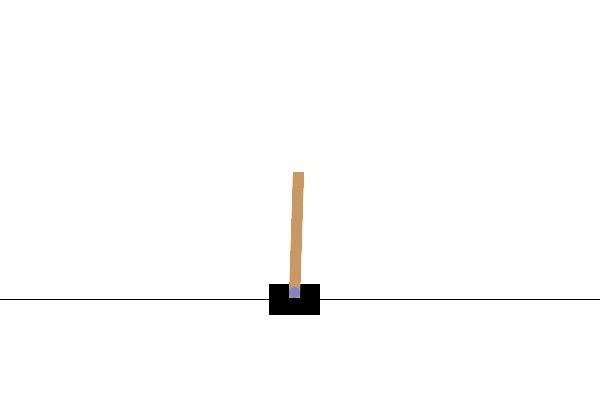
\includegraphics[width=0.85\linewidth]{pics/extracted_img-000.png}\par
            \scriptsize Σχ.\ 1: Το περιβάλλον \textlatin{CartPole}
        \end{column}
    \end{columns}
\end{frame}

% Slide 6 : Our Results 4 - Clean Reproduction P1 & P2
\begin{frame}{Τα Αποτελέσματά μας: Αναπαραγωγή Clean (Αρχές 1 \& 2)}
    \begin{columns}[onlytextwidth, T]
        \begin{column}{0.45\textwidth}
            \begin{itemize}
                \item \scriptsize \textbf{Παρατήρηση:} Σε καθαρές συνθήκες ($\sigma=0$), το \textlatin{Baseline} και η \textlatin{Αρχή 2} έχουν ταυτόσημη, εξαιρετικά υψηλή ακρίβεια.
                \item \scriptsize Η \textlatin{Αρχή 1} εμφανίζει ελαφρώς μεγαλύτερο σφάλμα (\textlatin{State MSE}).
                \item \scriptsize \textbf{Αιτιολογία:} Χωρίς οπτικές αλλοιώσεις, οι αρχιτεκτονικοί περιορισμοί (όπως το στενό \textlatin{bottleneck} των 4 διαστάσεων της Αρχής 1) απλώς περιορίζουν τη χωρητικότητα του δικτύου.
                \item \scriptsize Επιβεβαιώνεται ότι οι αρχές δεν στοχεύουν στην ακρίβεια υπό ιδανικές συνθήκες, αλλά στην ευρωστία.
            \end{itemize}
        \end{column}
        \begin{column}{0.52\textwidth}
            \centering
            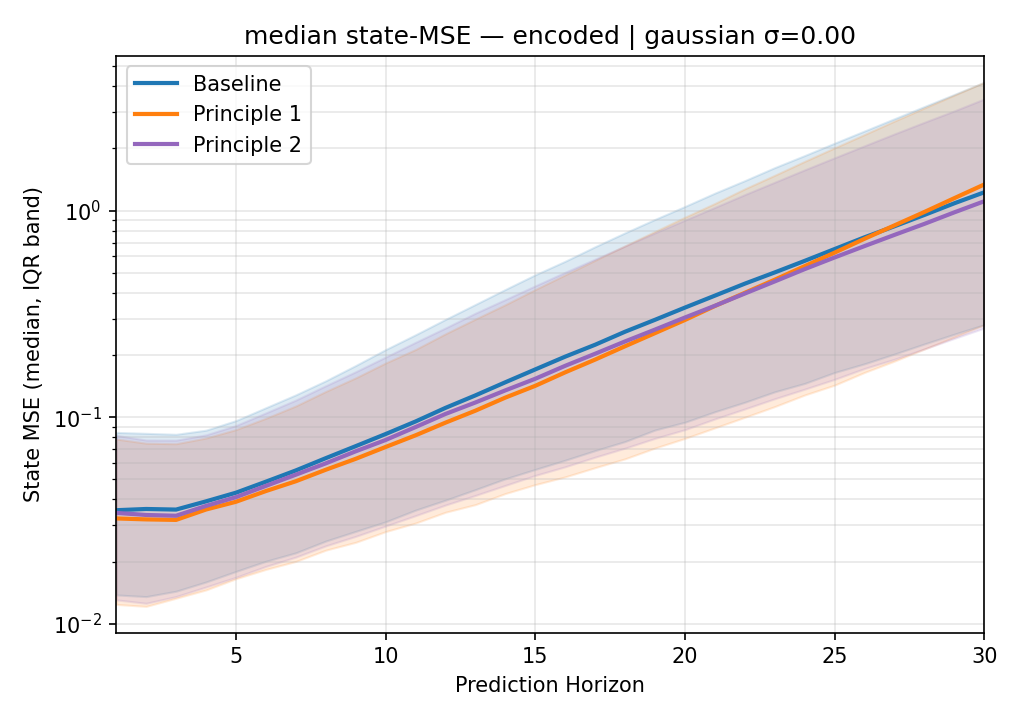
\includegraphics[width=0.95\linewidth]{pics/noise_median_iqr_encoded_gaussian_0p00_p1_p2.png}\par
            \scriptsize Σχ.\ 2: \textlatin{State MSE} σε καθαρό περιβάλλον ($\sigma=0.00$)
        \end{column}
    \end{columns}
\end{frame}

% Slide 7 : Our Results 5 - Clean Reproduction P3
\begin{frame}{Τα Αποτελέσματά μας: Αναπαραγωγή Clean (Αρχή 3)}
    \begin{columns}[onlytextwidth, T]
        \begin{column}{0.45\textwidth}
            \begin{itemize}
                \item \scriptsize \textbf{Παρατήρηση:} Υπό καθαρές συνθήκες, η πλήρης επίβλεψη (\textlatin{Baseline}) δίνει το χαμηλότερο δυνατό σφάλμα.
                \item \scriptsize Η ασθενής επίβλεψη (\textlatin{P3-weak}) ακολουθεί στενά.
                \item \scriptsize Η απουσία επίβλεψης ταχύτητας (\textlatin{P3-semi}) οδηγεί σε σημαντική συσσώρευση σφάλματος κατά το \textlatin{rollout}.
                \item \scriptsize \textbf{Συμπέρασμα:} Κάποια μορφή επίβλεψης ή φυσικής γνώσης για τις ταχύτητες είναι απαραίτητη για τη σταθεροποίηση της δυναμικής του \textlatin{World Model}.
            \end{itemize}
        \end{column}
        \begin{column}{0.52\textwidth}
            \centering
            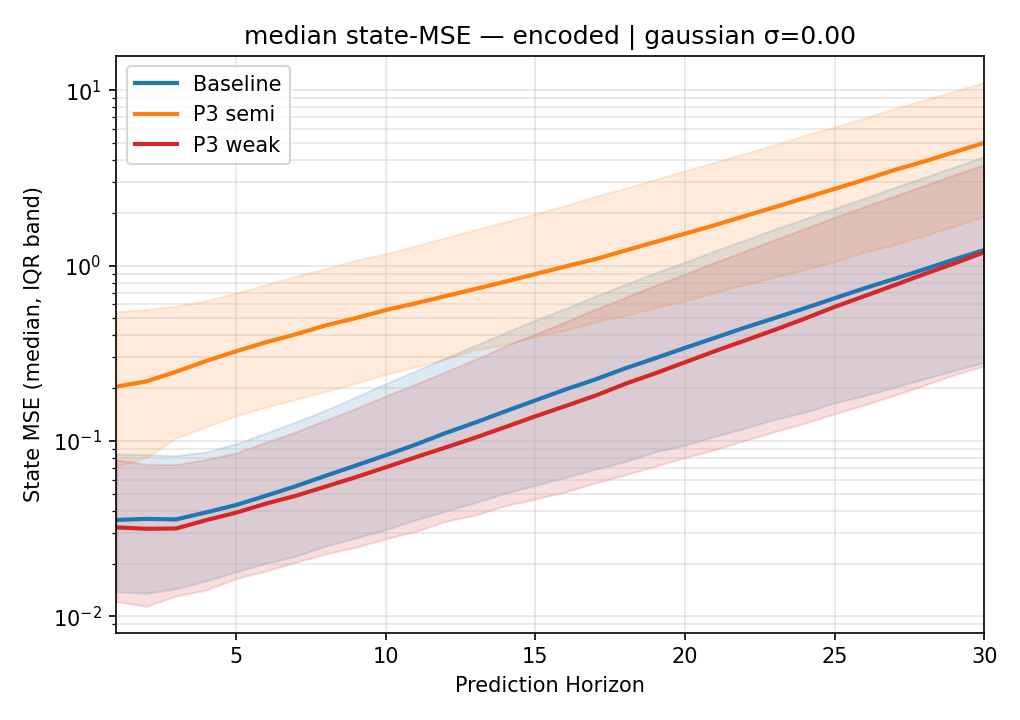
\includegraphics[width=0.95\linewidth]{pics/noise_median_iqr_encoded_gaussian_0p00_p3.png}\par
            \scriptsize Σχ.\ 3: Αξιολόγηση Αρχής 3 σε καθαρό περιβάλλον ($\sigma=0.00$)
        \end{column}
    \end{columns}
\end{frame}

% Slide 8 : Our Results 6 - OOD Stress-Testing Spatial Noise
\begin{frame}{Τα Αποτελέσματά μας: Ευρωστία σε Χωρικό Θόρυβο}
    \begin{columns}[onlytextwidth, T]
        \begin{column}{0.45\textwidth}
            \begin{itemize}
                \item \scriptsize \textbf{Η Αρχή 1 ως Δομικό Φίλτρο:} Παρουσιάζει εξαιρετική ευρωστία. Ακόμα και σε έντονο θόρυβο ($\sigma=0.30$), το \textlatin{MSE} παραμένει χαμηλό.
                \item \scriptsize Ο διαχωρισμός του \textlatin{encoder} εγκλωβίζει τον θόρυβο των \textlatin{pixels} στον κλάδο του στυλ ($z_{\text{\textlatin{img}}}$), προστατεύοντας τις φυσικές διαστάσεις ($z_{\text{\textlatin{phys}}}$).
                \item \scriptsize \textbf{Κατάρρευση της Αρχής 2:} Η κανονικοποίηση \textlatin{equivariance} αναγκάζει το μοντέλο να βασίζεται σε λεπτομερείς οπτικές δομές (ακμές). Όταν αυτές καταστρέφονται, ο \textlatin{encoder} παράγει ακραίες \textlatin{OOD} τιμές.
            \end{itemize}
        \end{column}
        \begin{column}{0.52\textwidth}
            \centering
            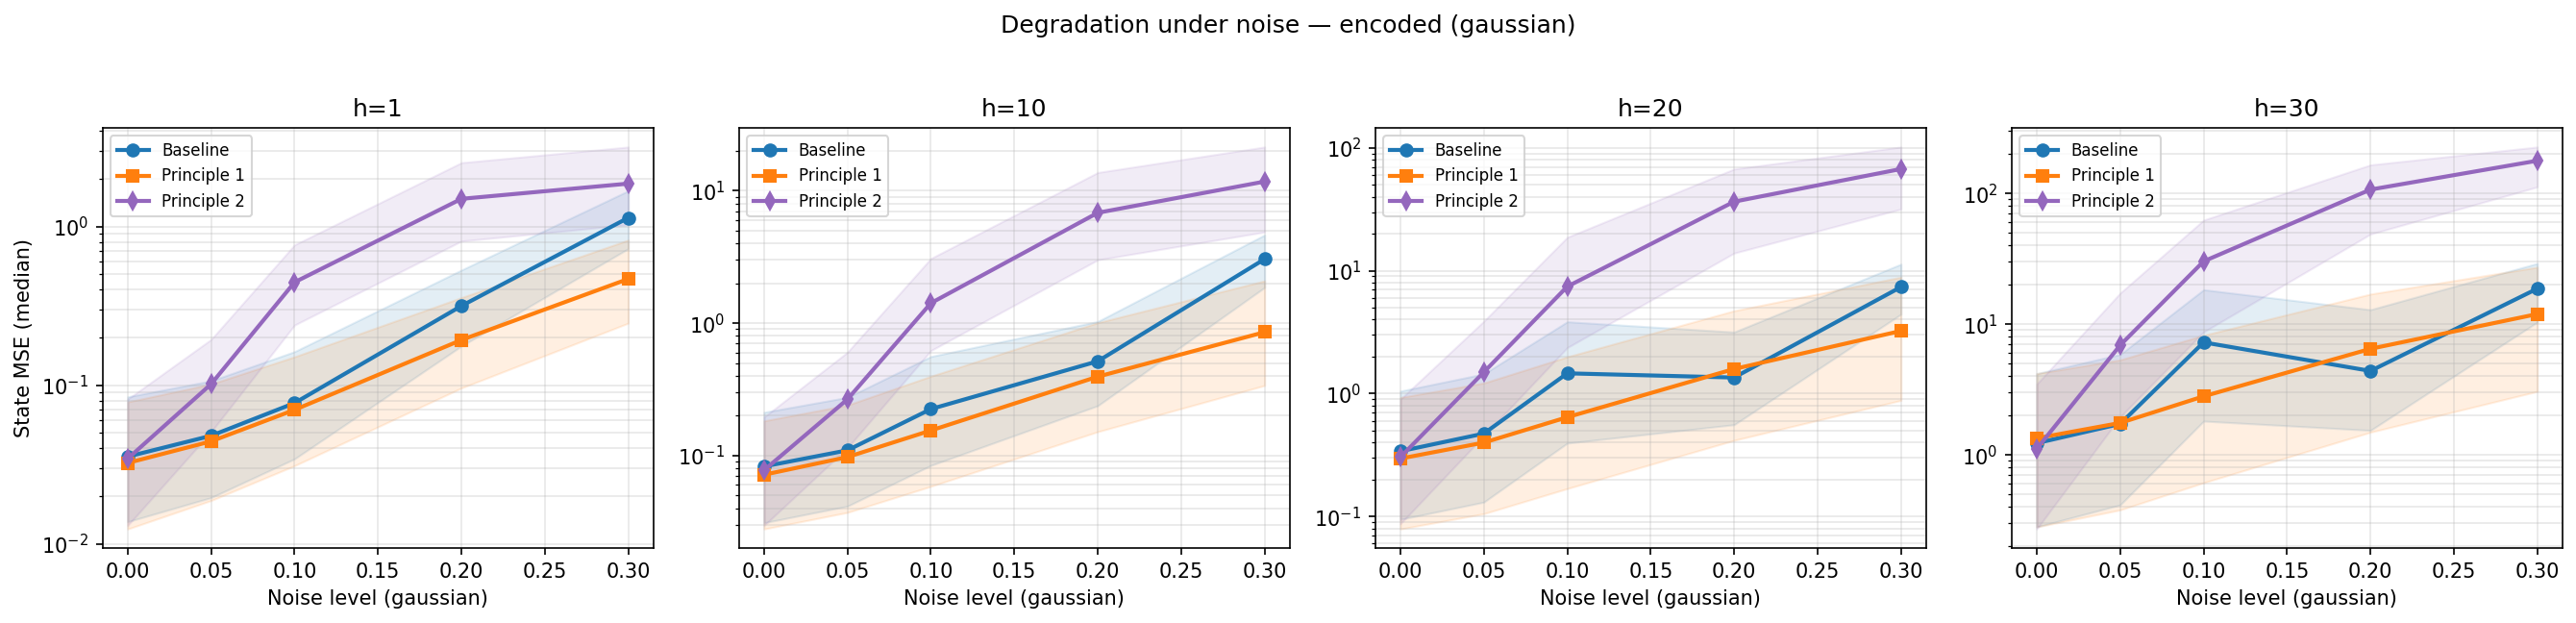
\includegraphics[width=0.95\linewidth]{pics/noise_degradation_encoded_gaussian.png}\par
            \scriptsize Σχ.\ 4: Ευρωστία σε \textlatin{Gaussian Noise} ($h=30$)
        \end{column}
    \end{columns}
\end{frame}

% Slide 9 : Our Results 7 - OOD Stress-Testing Brightness Jitter
\begin{frame}{Τα Αποτελέσματά μας: Ευρωστία σε Φωτεινότητα}
    \begin{columns}[onlytextwidth, T]
        \begin{column}{0.45\textwidth}
            \begin{itemize}
                \item \scriptsize \textbf{Η Αρχή 2 ως Ασπίδα Φωτισμού:} Όταν εφαρμόζεται μεταβολή φωτεινότητας, η Αρχή 2 υπερτερεί ξεκάθαρα του \textlatin{Baseline}.
                \item \scriptsize \textbf{Στατιστική Επαλήθευση:} Η ανάλυση \textlatin{paired bootstrap} δείχνει ότι η διαφορά $\Delta = \text{\textlatin{Baseline}} - \text{\textlatin{Principle 2}}$ είναι σταθερά θετική με 95\% διάστημα εμπιστοσύνης.
                \item \scriptsize \textbf{Εξήγηση:} Η ρητή κανονικοποίηση αναγκάζει τον \textlatin{encoder} να αγνοεί τις ομοιόμορφες μεταβολές χρώματος/φωτισμού, διατηρώντας αναλλοίωτη τη φυσική κατάσταση.
            \end{itemize}
        \end{column}
        \begin{column}{0.52\textwidth}
            \centering
            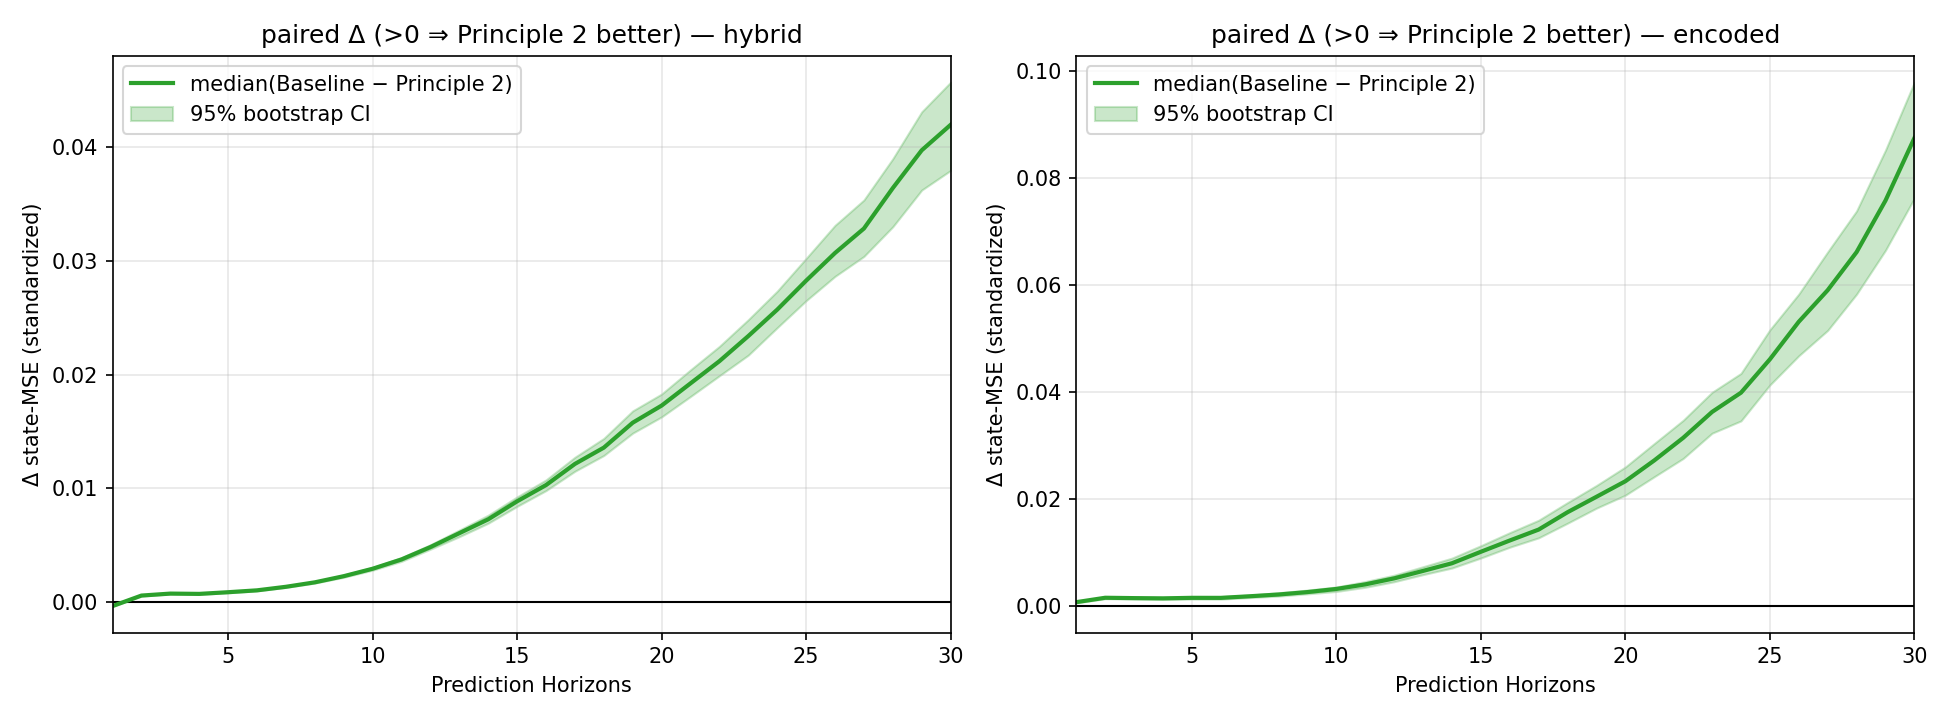
\includegraphics[width=0.95\linewidth]{pics/cmp_paired_diff.png}\par
            \scriptsize Σχ.\ 5: \textlatin{Paired Difference} υπό \textlatin{Brightness Jitter}
        \end{column}
    \end{columns}
\end{frame}

% Slide 10 : Our Results 8 - Weak Supervision under Noise
\begin{frame}{Τα Αποτελέσματά μας: Ασθενής Επίβλεψη υπό Θόρυβο}
    \begin{columns}[onlytextwidth, T]
        \begin{column}{0.46\textwidth}
            \begin{block}{Το Παράδοξο της Αρχής 3}
                \begin{itemize}
                    \item \scriptsize Υπό χωρικό θόρυβο, η ασθενής επίβλεψη (\textlatin{P3-weak}) \textbf{υπερτερεί} του πλήρως επιβλεπόμενου \textlatin{Baseline}.
                    \item \scriptsize \textbf{Εξήγηση:} οι «θορυβώδεις» εκτιμήσεις ταχυτήτων (πεπερασμένες διαφορές) δρουν ως έμμεση κανονικοποίηση (\textlatin{implicit regularizer}), αποτρέποντας \textlatin{overfit} στις καθαρές λεπτομέρειες.
                \end{itemize}
            \end{block}
            \setbeamercolor{block title}{bg=accentorange}
            \begin{block}{Συμπέρασμα}
                \scriptsize Η απαίτηση για τέλεια δεδομένα επίβλεψης είναι μύθος: η προσεγγιστική επίβλεψη καθιστά το μοντέλο πιο εύρωστο εκτός κατανομής.
            \end{block}
        \end{column}
        \begin{column}{0.52\textwidth}
            \centering
            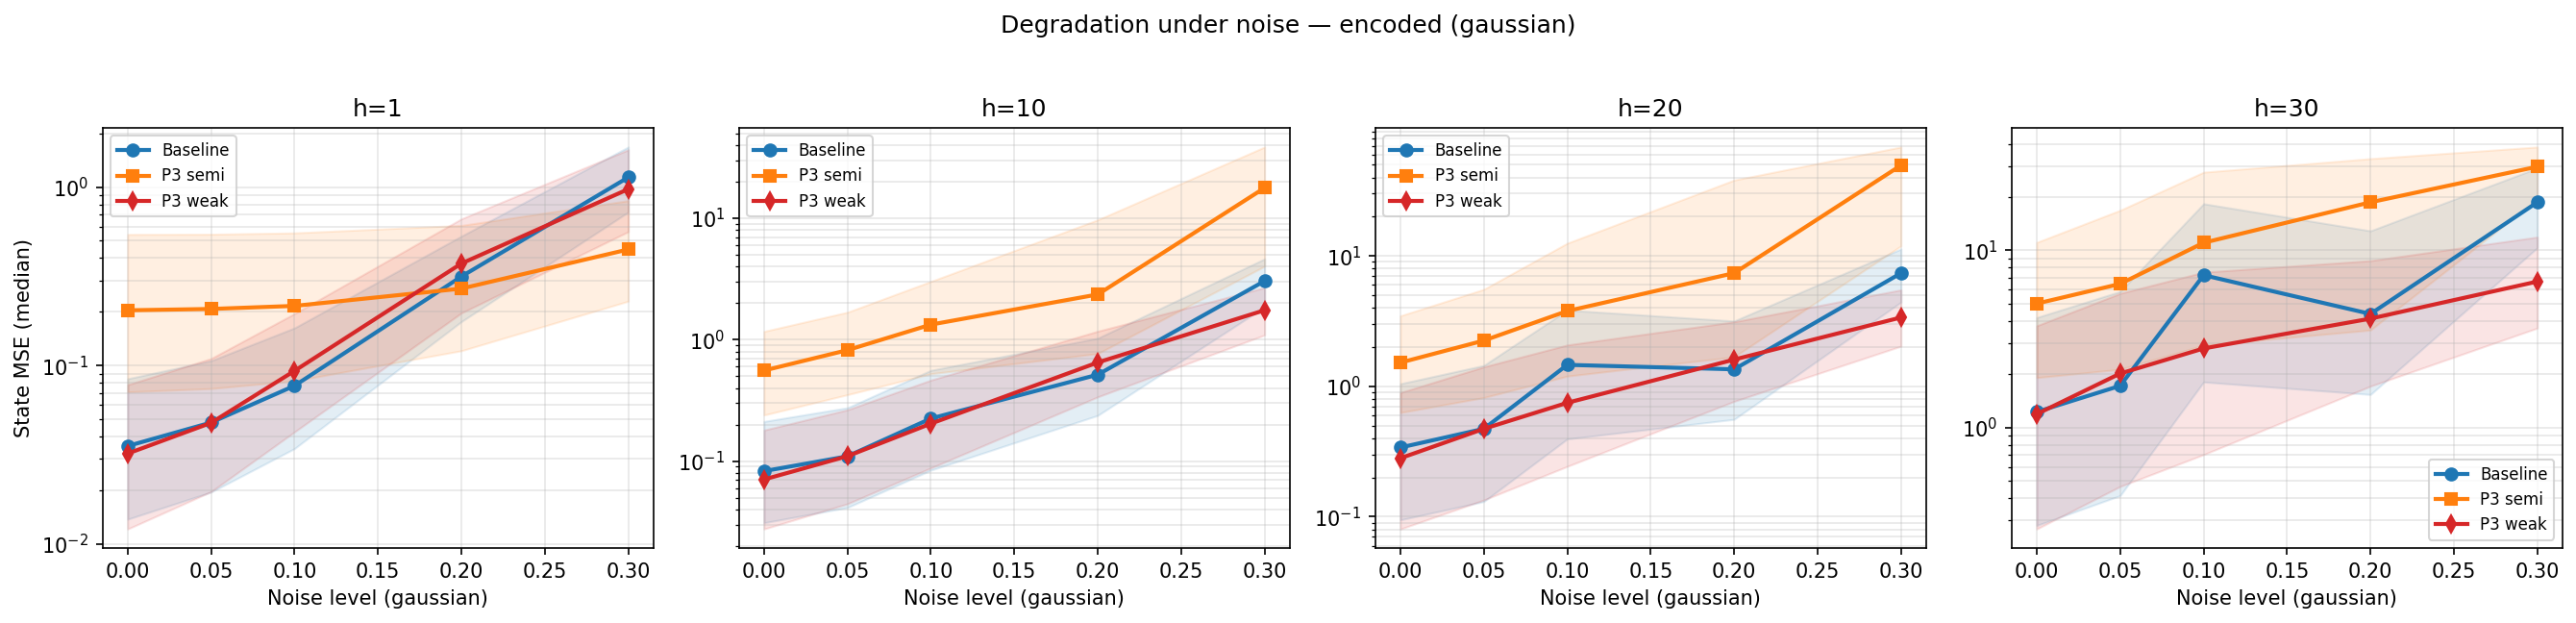
\includegraphics[width=0.99\linewidth]{pics/p3_noise_degradation.png}\par
            \scriptsize Σχ.\ 6: Αρχή 3 υπό \textlatin{Gaussian noise}. Σε υψηλό θόρυβο/ορίζοντα η \textlatin{P3-weak} (κόκκινο) πέφτει κάτω από το \textlatin{Baseline} (μπλε).
        \end{column}
    \end{columns}
\end{frame}

% Slide 10b : Our Results 9 - P4 Compositional Decoding (Αρχή 4)
\begin{frame}{Τα Αποτελέσματά μας: Διαμέριση Εξόδου (Αρχή 4)}
    \begin{columns}[onlytextwidth, T]
        \begin{column}{0.46\textwidth}
            \begin{itemize}
                \item \scriptsize \textbf{Ιδέα:} Αντικατάσταση του μονολιθικού \textlatin{decoder} με τρεις μικρούς, ανεξάρτητους αποκωδικοποιητές (\textlatin{cart}, \textlatin{pole}, \textlatin{background}).
                \item \scriptsize \textbf{Αποτέλεσμα:} \alert{$-75.4\%$} παράμετροι \textlatin{decoder} (\textlatin{665k} $\to$ \textlatin{164k}) και $-25.9\%$ συνολικά, με \emph{ταυτόσημη} ποιότητα ανακατασκευής.
                \item \scriptsize Επιβεβαιώνεται ο ισχυρισμός του \textlatin{paper}: η συνθετικότητα μειώνει δραστικά το μέγεθος χωρίς απώλεια ποιότητας, διευκολύνοντας την επαλήθευση ανά αντικείμενο.
            \end{itemize}
            \vspace{0.1cm}
            \centering\scriptsize
            \begin{tabular}{l r r}
                \toprule
                \textlatin{Metric} & \textlatin{Baseline} & \textlatin{P4} \\
                \midrule
                \textlatin{recon MSE} $\downarrow$ & 0.00315 & 0.00306 \\
                \textlatin{SSIM} $\uparrow$ & 0.9581 & 0.9582 \\
                \textlatin{decoder params} $\downarrow$ & \textlatin{665k} & \textbf{\textlatin{164k}} \\
                \bottomrule
            \end{tabular}
        \end{column}
        \begin{column}{0.52\textwidth}
            \centering
            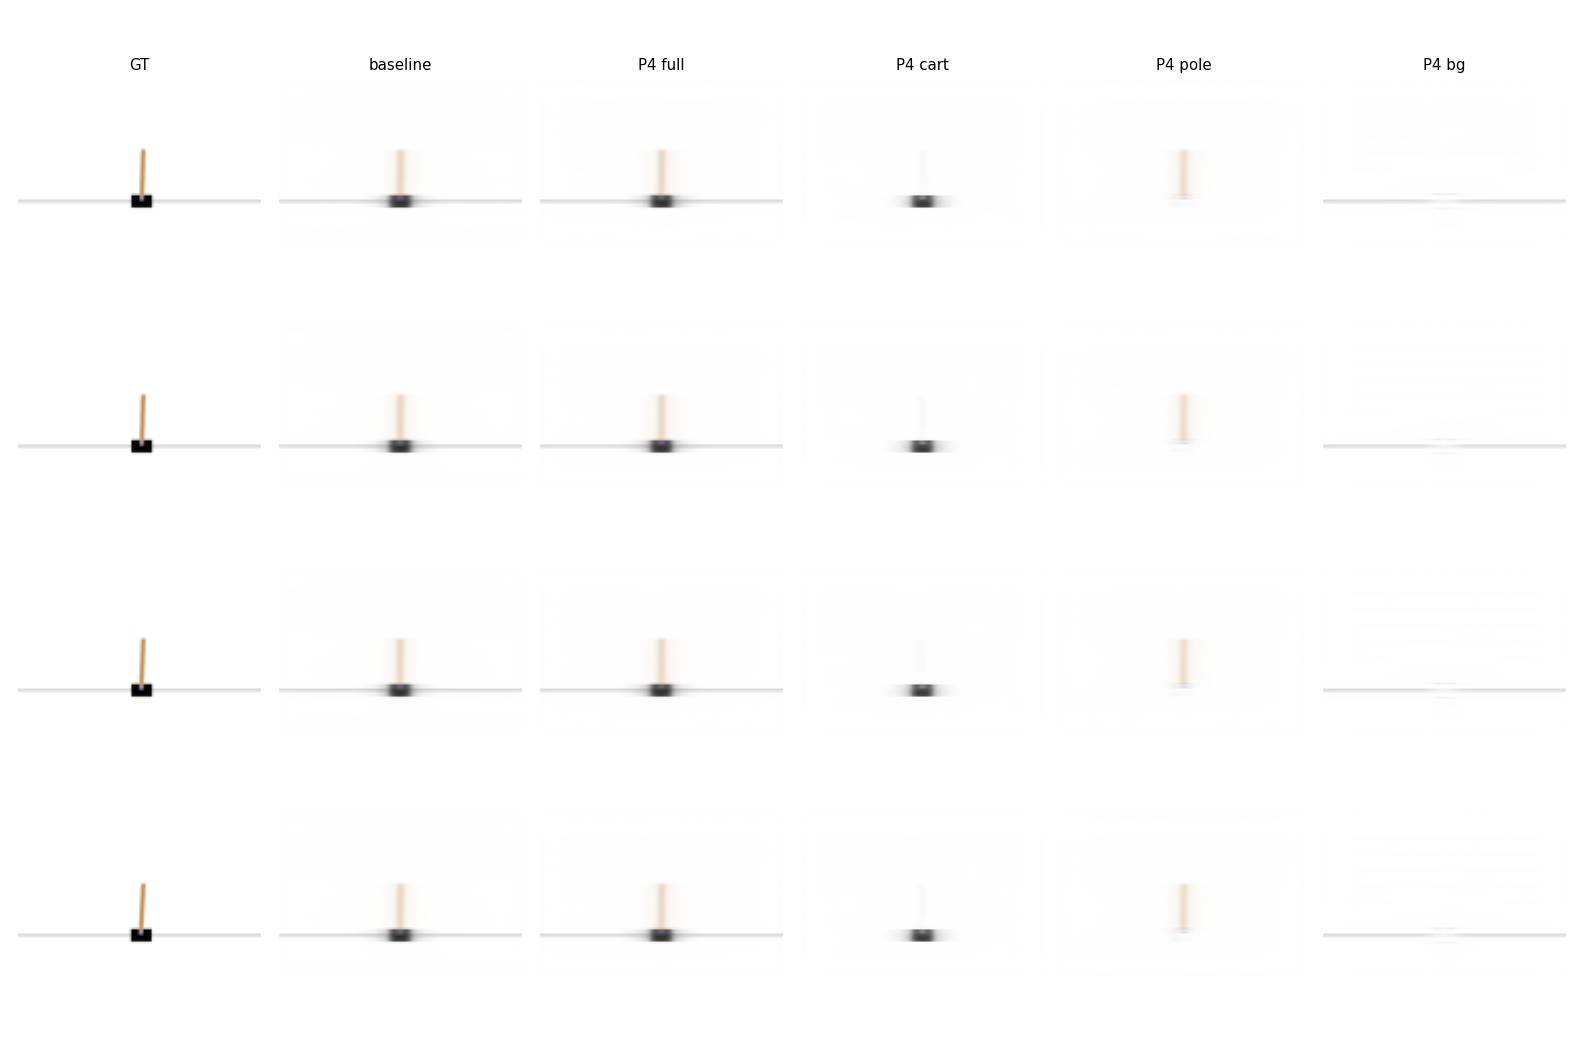
\includegraphics[width=0.99\linewidth]{pics/p4_compare.png}\par
            \scriptsize Σχ.\ 7: \textlatin{GT} vs \textlatin{baseline} vs \textlatin{P4} (σύνθεση \& επιμέρους \textlatin{cart}/\textlatin{pole}/\textlatin{bg}).
        \end{column}
    \end{columns}
\end{frame}

% Slide 10c : Beyond-paper extension - Interpretable Dynamics with SINDy
\begin{frame}{Επέκταση πέρα από το \textlatin{Paper}: Ερμηνεύσιμη Δυναμική (\textlatin{SINDy})}
    \footnotesize Αν ο λανθάνων χώρος είναι όντως φυσικός, τότε και η \emph{δυναμική} του πρέπει να γράφεται ως αραιή εξίσωση — όχι «μαύρο κουτί». Εφαρμόσαμε \textlatin{SINDYc} στις φυσικές διαστάσεις και το συγκρίναμε με το \textlatin{LSTM} και ένα \textlatin{gray-box hybrid} (\textlatin{SINDy} + υπολειμματικό \textlatin{LSTM}).\par\vspace{0.15cm}
    \begin{columns}[onlytextwidth, T]
        \begin{column}{0.48\textwidth}
            \begin{block}{Ανακαλυφθείσες εξισώσεις (12 όροι / 88)}
                \scriptsize
                \[ x_{t+1} = x_t + 0.021\,\dot{x} \]
                \[ \theta_{t+1} = \theta_t + 0.176\,\dot{\theta} \]
                \scriptsize Ανακτώνται \emph{αυτόματα} τα κινηματικά ολοκληρώματα και ο όρος βαρύτητας $\sin\theta$ — ρητή, αναγνώσιμη φυσική.
            \end{block}
        \end{column}
        \begin{column}{0.48\textwidth}
            \scriptsize \textbf{Ευρωστία σε θόρυβο} (\textlatin{mean State MSE}, \textlatin{Baseline}):
            \par\vspace{0.1cm}\centering
            \begin{tabular}{l r r r}
                \toprule
                $\sigma$ & \textlatin{LSTM} & \textlatin{SINDy} & \textlatin{Hybrid} \\
                \midrule
                $0.00$ & $0.033$ & $0.035$ & $\mathbf{0.027}$ \\
                $0.30$ & $0.509$ & $\mathbf{0.130}$ & $0.441$ \\
                \bottomrule
            \end{tabular}
            \par\vspace{0.15cm}
            \raggedright\scriptsize Στο $\sigma=0.30$ το \textlatin{SINDy} υποβαθμίζεται $\times 3.7$ ενώ το \textlatin{LSTM} $\times 15$: η φυσική δομή δίνει ευρωστία και ερμηνευσιμότητα με $\sim$12 μόνο συντελεστές.
        \end{column}
    \end{columns}
\end{frame}

% ==========================================
% SECTION 3: ΑΠΟΤΙΜΗΣΗ & ΕΠΕΚΤΑΣΕΙΣ (1-2 διαφάνειες)
% ==========================================

% Slide 11 : Evaluation & Future Extensions
\begin{frame}{Αποτίμηση \& Μελλοντικές Επεκτάσεις}
    \begin{columns}[onlytextwidth, T]
        \begin{column}{0.48\textwidth}
            \begin{block}{Αποτίμηση}
                \begin{itemize}
                    \item \scriptsize \textbf{Αποσύνδεση (Αρχή 1):} Η ασφαλέστερη επιλογή για γενικό χωρικό θόρυβο.
                    \item \scriptsize \textbf{Equivariance (Αρχή 2):} Εξαιρετική για συγκεκριμένες μεταβολές (φωτισμός), αλλά εύθραυστη σε θόρυβο pixel.
                    \item \scriptsize \textbf{Ασθενής Επίβλεψη (Αρχή 3):} Προσφέρει regularizing effect OOD.
                \end{itemize}
            \end{block}
        \end{column}
        \begin{column}{0.48\textwidth}
            \begin{block}{Μελλοντικές Επεκτάσεις}
                \begin{itemize}
                    \item \scriptsize \textbf{Ερμηνεύσιμη δυναμική:} επέκταση από \textlatin{SINDy} σε \textlatin{Hamiltonian/Lagrangian NNs} για δυναμική που διατηρεί την ενέργεια.
                    \item \scriptsize \textbf{Φυσικοί Κανόνες από \textlatin{LLMs}:} αυτόματος εντοπισμός κανόνων \textlatin{equivariance/invariance}.
                    \item \scriptsize \textbf{Σύνδεση με Έλεγχο:} ενσωμάτωση του ερμηνεύσιμου $z_{\text{phys}}$ σε ελεγκτές \textlatin{MPC} για ασφαλές \textlatin{planning}.
                \end{itemize}
            \end{block}
        \end{column}
    \end{columns}
\end{frame}

% ==========================================
% SECTION 4: ΚΑΤΑΝΟΜΗ ΕΡΓΑΣΙΩΝ (πίνακας 1 διαφάνεια)
% ==========================================

% Slide 12 : Team & Roles Table
\begin{frame}{Κατανομή Εργασιών \& Ρόλοι Μελών}
    \centering
    \renewcommand{\arraystretch}{1.25}
    \footnotesize
    \begin{tabular}{l l p{7.5cm}}
        \toprule
        \textbf{Μέλος Ομάδας} & \textbf{ΑΜ} & \textbf{Ρόλος \& Συνεισφορά στην Εργασία} \\
        \midrule
        \textbf{Πλουμής Φίλιππος} & 03122115 & Συλλογή δεδομένων, pipeline μεταφοράς στα μοντέλα. \\
        \textbf{Ρήγας Αθανάσιος} & 03122078 & VAE/LSTM updates, Scheduled Sampling, Curriculum Learning, επέκταση SINDy / gray-box hybrid \& noise sweep. \\
        \textbf{Μπακογιώργος Ηλίας} & 03122019 & Υλοποίηση Αρχής 1 (disentanglement) \& Αρχής 2 (equivariance). \\
        \textbf{Φειδάκης Αθανάσιος} & 03122676 & Υλοποίηση Αρχής 3 (supervision), Αρχής 4 \& paired bootstrap eval. \\
        \bottomrule
    \end{tabular}
    \vspace{0.4cm}
    \begin{block}{Συνεργασία}
        \scriptsize Όλα τα μέλη συμμετείχαν εξίσου στη θεωρητική μελέτη του άρθρου, στο σχεδιασμό των OOD stress-tests,\\ στη συγγραφή της τελικής αναφοράς και στην προετοιμασία της παρουσίασης.
    \end{block}
\end{frame}

% ==========================================
% SECTION 5: RETROSPECTIVE (1 διαφάνεια)
% ==========================================

% Slide 13 : Retrospective
\begin{frame}{Retrospective: Τι μας δυσκόλεψε}
    \begin{columns}[onlytextwidth, T]
        \begin{column}{0.48\textwidth}
            \begin{block}{Τι μας δυσκόλεψε}
                \begin{itemize}
                    \item \scriptsize \textbf{Ποιότητα Αρχικού Κώδικα:} Ο κώδικας του paper ήταν εξαιρετικά ελλιπής, χωρίς scheduled sampling ή curriculum, αναγκάζοντάς μας να ξαναγράψουμε μεγάλο μέρος του.
                    \item \scriptsize \textbf{Multi-Objective Loss:} Η ισορροπία μεταξύ ανακατασκευής (\textlatin{ELBO}), equivariance (\textlatin{loss}) και επίβλεψης ήταν πολύ ευαίσθητη και απαιτούσε επίπονο \textlatin{tuning}.
                \end{itemize}
            \end{block}
        \end{column}
        \begin{column}{0.48\textwidth}
            \setbeamercolor{block title}{bg=accentorange}
            \begin{block}{Τι θα κάναμε καλύτερα}
                \begin{itemize}
                    \item \scriptsize \textbf{Automated Hyperparameter Tuning:} Χρήση βιβλιοθηκών (π.χ. \textlatin{Optuna}) για την αυτόματη εύρεση των βαρών $\lambda$ της απώλειας.
                    \item \scriptsize \textbf{Νωρίτερη OOD Αξιολόγηση:} Αν είχαμε εισάγει το θόρυβο νωρίτερα, θα είχαμε εντοπίσει τις αδυναμίες της Αρχής 2 πριν επενδύσουμε χρόνο στο setup της.
                \end{itemize}
            \end{block}
        \end{column}
    \end{columns}
    \vspace{0.3cm}
    \centering\footnotesize\textit{Ευχαριστούμε για την προσοχή σας. Είμαστε στη διάθεσή σας για ερωτήσεις.}
\end{frame}

\end{document}
